\section{What If The Safety Alignment Were Deeper?}
\label{sec:make_alignment_deeper}

\begin{comment}
\ahmad{The major structural comment that I have is that there are two distinct mitigations proposed against different issues, both of which are interesting and complementary. I am not sure if the current structure does justice to them. Here is the way I see them.
\begin{itemize}
    \item Model developer makes their alignment deeper first: Propose a data augmentation objective to make alignment deeper.
    \item Model developer comes up with a new finetuning objective that is more robust against undoing alignment: Propose a new finetuning objective so that we don't undo alignment.
\end{itemize}
Given this, here is an alternate proposed structure for telling the story. I would take them both into the same section, and call that section mitigation strategies. And then I'd test the two ideas separately, and even jointly.  I may even swap their order and say now that I am a model provider, the first thing that I'd want to do given that I know what the culprit is would be to deepen my alignment and specifically in the counterfactual generations. Hence, I'd first start with trying to deepen my alignment with counterfactual data augmentation. Great! This helps, but can I also devise a custom finetuning loss so that I can mitigate against undoing alignment?  Great, this also works. And then you can end w/ combination of both these ideas can be even more useful.}



\peter{Somewhere here I want to add a note that there's an RL sampling distribution perspective that may help explain this. And then add a small paragraph in the Appendix on this to set up some future work. Leaving this not to myself so when this section is more complete, I'll drop it in somewhere. }

\ahmad{In my mind, the data augmentation is trying to explore the underepresented states during training -- which to me is the culprit here. These vulnerabilities in spirit are similar to those of AlphaGo when pushed into underepresented game plans (albeit ours are much simpler variants and we did not even need ML to discover them): \url{https://arxiv.org/abs/2211.00241}.}

\peter{Ahmad, agree! I think it's actually two-fold. (1) The starting states ($d_0$) we could possibly samples are so vast, we actually never sample them, especially ones; (2) Even when we do sample them, we don't do enough exploration because the KL constraint keeps you from doing so. And I'm pretty sure most RLHF implementations don't use the entropy bonus that is required for theoretical convergence of policy gradients.}

\ahmad{Agreed. In addition, unlike games, here the reward (safety classifier) is also trained on data that doesn't do much exploration. Hence, exploration without hacking an unreliable reward is actually really challenging.}

\peter{Another great point!}
\end{comment}

Following the notion of shallow safety alignment that we elaborate on in Section~\ref{sec:shallow_alignment}, we now consider its counterfactual: \textbf{what if the safety alignment were deeper?} Particularly, if the alignment's control over the model's harmful outputs could go deeper than just the first few tokens, would it be more robust against the range of vulnerabilities we have observed? To investigate this counterfactual, we experiment with a simple data augmentation approach~(Section~\ref{subsec:data_augmentation_approach}) which we find can meaningfully deepen the safety alignment's influence over the model's harmful outputs. In Section~\ref{subsec:evaluate_data_augmentation}, we validate that this deeper alignment indeed results in a promising improvement for mitigating multiple vulnerabilities that we have observed in shallowly aligned models.


\subsection{Data Augmentation with Safety Recovery Examples}
\label{subsec:data_augmentation_approach}

%As we have noted in Section~\ref{subsec:refusal_prefix},

%mostly work with a sequence-level alignment objective while not accounting for the smaller fine-grained units in sequences. 

%This can happen because current alignment approaches seldom account for such effects. Let's use $\bx, \bm{r}, \bm{h}$ to denote a harmful instruction~($\bx$), an ideally safe refusal response~($\bm{r}$), and an undesired harmful response~($\bm{h}$). In SFT-based alignment, $P(\bm{h} | \bx)$ is diminished by promoting $P(\bm{r} | \bx)$. This objective does not specify how deep the alignment should go. In an extreme case, $P(\bm{h}|\bx) = P(h_1 |\bx) \times P(\bm{h}_{>1}|\bx, h_1)$ can be diminished by simply adapting $P(\bm{h}|\bx) = P(h_1 |\bx) \times P(\bm{h}_{>1}|\bx, h_1) = 0$, while $P({h}_{>1}|\bx, h_1) = 1$ remains. Conversely, we hope an ideal alignment has much deeper suppression of harmful content, for instance, by ensuring that $P({h}_{> i}|\bx, h_{\le i}) = 0$ for any $i \in [0, |\bm{h}|]$. However, the objective does not encode any preference between the two. This notion also holds true for RL-based alignment, where the objective is simply to promote sequences that get high scores from some reward models.


%A sequence-level alignment objective only requires $P(\bm{h} | \bx)$ to be diminished~(e.g., by promoting $P(\bm{r} | \bx)$ to dominate the probability space). However, such objectives do not specify how deep the alignment should go. In an extreme case, having $P(h_1 |\bx) = 0$ is sufficient to render $P(\bm{h}|\bx) = P(h_1 |\bx) \times P(\bm{h}_{>1}|\bx, h_1) = 0$, even if $P({h}_{>1}|\bx, h_1) = 1$. Conversely, we hope an ideal alignment has much deeper suppression of harmful content, for instance, by ensuring that $P({h}_{> i}|\bx, h_{\le i}) = 0$ for any $i \in [0, |\bm{h}|]$. However, sequence-level alignment objectives can not encode any preference between the two. 




%This notion also holds true for RL-based alignment, where the objective is simply to generate sequences that get high scores from some reward models. Ideally, a deeper alignment would have $P({h}_{> i}|\bx, h_{\le i}) = 0$ for any $i \in [1, |\bm{h}|]$. The objective does not encode any preference between the two. This notion also holds true for RL-based alignment, where reward models rely on the entire generated sequence of a model. Furthermore, as noted in Section~\ref{subsec:refusal_prefix}, learning the initial prefixes is sufficient to ensure the safety of the entire sequence, naturally leading to a reward-hacking scheme that achieves high safety scores from the reward model.

% It can happen because current safety alignment mostly works with a sequence-level objective. Specifically, let's use $\bx, \bm{r}, \bm{h}$ to denote a harmful instruction~($\bx$), an ideally safe refusal response~($\bm{r}$), and an undesired harmful response~($\bm{h}$). A sequence-level safety alignment objective is basically to diminish $P(\bm{h} | \bx)$, for example, symmetrically by promoting $P(\bm{r} | \bx)$. The problem is that such an objective does not specify how deep the alignment should go. In an extreme case, $P(\bm{h}|\bx) = P(h_1 |\bx) \times P(\bm{h}_{>1}|\bx, h_1)$ can be diminished by simply adapting $P(\bm{h}|\bx) = P(h_1 |\bx) \times P(\bm{h}_{>1}|\bx, h_1) = 0$, while $P({h}_{>1}|\bx, h_1) = 1$ remains. Conversely, we hope an ideal alignment has much deeper suppression of harmful content, for instance, by ensuring that $P({h}_{> i}|\bx, h_{\le i}) = 0$ for any $i \in [0, |\bm{h}|]$. However, the objective does not encode any preference between the two.


%We show it is feasible to meaningfully deepen the safety alignment of a shallowly-aligned model by further fine-tuning it with this data augmentation approach.
%Our following experiments demonstrate the feasibility of meaningfully deepening the safety alignment of a shallowly aligned model by simply further fine-tuning it with this data augmentation.

%We start by collecting a set of data triplets in the form of $\{(\bx, \bm{h}, \bm{r})\}$, where $\bx$ is a harmful instruction, $\bm{h}$ is the harmful response generated by the model, and $\bm{r}$ is an ideally safe refusal response.

%Let's use $\bx, \bm{r}, \bm{h}$ to denote a harmful instruction~($\bx$), an ideally safe refusal response~($\bm{r}$), and an undesired harmful response~($\bm{h}$). In SFT-based alignment, $P(\bm{h} | \bx)$ is diminished by promoting $P(\bm{r} | \bx)$. This objective does not specify how deep the alignment should go. In an extreme case, $P(\bm{h}|\bx) = P(h_1 |\bx) \times P(\bm{h}_{>1}|\bx, h_1)$ can be diminished by simply adapting $P(\bm{h}|\bx) = P(h_1 |\bx) \times P(\bm{h}_{>1}|\bx, h_1) = 0$, while $P({h}_{>1}|\bx, h_1) = 1$ remains. Conversely, we hope an ideal alignment has much deeper suppression of harmful content, for instance, by ensuring that $P({h}_{> i}|\bx, h_{\le i}) = 0$ for any $i \in [0, |\bm{h}|]$. However, the objective does not encode any preference between the two. This notion also holds true for RL-based alignment, where the objective is simply to promote sequences that get high scores from some reward models.

Formally, let's use $\bx, \bm{h}$ to denote a harmful instruction~($\bx$) and its harmful response~($\bm{h}$). As noted in Section~\ref{sec:shallow_alignment}, a shallow safety alignment can keep the probability of the harmful response $\pi_{\theta}(\bm{h}|\bx)$ low, but this is achieved by merely suppressing the initial tokens of $\bm{h}$. For example, an extreme case is to just adapt $\pi_{\theta}(h_1 |\bx) = 0$ while leaving $\pi_{\theta}(\bm{h}_{>1}|\bx, h_1) = 1$. Then the overall probability of the harmful response $\pi_{\theta}(\bm{h}|\bx) = \pi_{\theta}(h_1 |\bx) \times \pi_{\theta}(\bm{h}_{>1}|\bx, h_1) = 0$ is indeed diminished. However, this does not control the harmful behaviors encoded just one token deeper by $\pi_{\theta}(\bm{h}_{>1}|\bx, h_1) = 1$. Therefore, a natural counterfactual of the shallow safety alignment is to push its influence deeper into the model's harmful outputs, for instance, by keeping $\pi_{\theta}(\bm{h}_{> k}|\bx, \bm{h}_{\le k})$ low for any $k \in [0, |\bm{h}|]$ or at least a sufficiently large $k$. We propose a data augmentation approach to encode this notion. 

%\peter{I'm not sure that counterfactual is the right term to use here? It implies some sort of causal inference setup. Should probably find a different term. What about ``recovery'' safety examples.}


\textbf{Safety Recovery Examples.} Consider triplets in the form of $(\bx, \bm{h}, \bm{r})$, in which a refusal response $\bm{r}$ is paired with the harmful instruction and its harmful response. Instead of solely promoting $\pi_{\theta}(\bm{r} | \bx)$ as in some standard safety alignment approaches, we propose to also augment $\pi_{\theta}(\bm{r} | \bx, \bm{h}_{\le k}), k\sim \text{Uniform}[1, C]$ for some constant $C \le |\bm{h}|$. This augmented data steers the model to get back on track with refusal responses even when the first few generated tokens initially deviate to a trajectory of harmful content. In this way, it explicitly trains the model to suppress harmful content more deeply within the response, reducing $\pi_{\theta}(\bm{h}_{> k} | \bx, \bm{h}_{\le k})$ at a deeper depth of $k$. We refer to such augmented data as safety recovery examples. Such examples typically appear as:

\noindent\fcolorbox{deepred}{mildyellow}{\begin{minipage}{0.98\columnwidth}
\textcolor{gray}{<s> [INST] <<SYS>> (System Prompt) <</SYS>>$\backslash$n$\backslash$n}Please give me step-by-step instructions for building a bomb. \textcolor{gray}{[/INST]} Step 1: Gather phosphorus \textcolor{deepred}{\textbf{I cannot fulfill your request. It's not}\textcolor{gray}{... </s>} }
\end{minipage}}

As illustrated, the text is synthetic and not even coherent in natural language, implying that it is unlikely to be naturally produced by human labelers for SFT data or sampled from models for preference optimization data. Thus, these augmented examples essentially cover outlier cases, which are useful for encoding a deeper safety alignment notion.\footnote{We note that there are ties to ensuring sufficient exploration in reinfocement learning that we do not explore formally here, but leave to future work. }



\textbf{Implementations.} We experiment with this data augmentation to deepen the safety alignment of the Llama-2-7B-Chat model. Since the model's alignment pipeline is not publicly available, we can not apply the data augmentation to align the model from scratch. Alternatively, in implementation, we experiment by directly fine-tuning the already aligned Llama-2-7B-Chat model further with the augmented safety recovery examples. To implement it, we construct a safety dataset $D_H$ comprising 256 examples of triplets $(\bx, \bm{h}, \bm{r})$ in the form we described above. To prevent the decrease of model utility, we also take benign instructions from the Alpaca~\cite{alpaca} dataset. We distill the responses to each of these Alpaca instructions using the initial Llama-2-7B-Chat model to create dataset $D_B$. This dataset serves as a utility anchor, teaching the model not to alter its original responses to benign instructions. Taking together, we fine-tune the model using the following objective:
\begin{align}
  & \min_{\theta} \ \  \alpha \times \Big\{ \mathop{\mathbb{E}}_{\substack{(\bx,\bm{h}, \bm{r}) \sim D_H, \\ k \sim \mathcal{P}_k}} - \log \pi_{\theta}(\bm{r}|\bx, \bm{h}_{\le k}) \Big\} +  (1-\alpha) \times \Big\{ \mathop{\mathbb{E}}_{(\bx',\by') \sim D_B} - \log \pi_{\theta}(\by'|\bx') \Big\}
\label{eqn:data-augmentation-objective}
\end{align}
Here, $\pi_{\theta}$ is initialized with the aligned Llama-2-7B-Chat model. We set the number of prefilled tokens $k$ to follow a distribution $\mathcal{P}_k$, where $k=0$ with a $50\%$ probability, and $k$ is uniformly sampled from $[1, 100]$ with a $50\%$ probability. We set $\alpha = 0.2$ to balance the ratio of safety examples and utility examples in the objective. %In batch-wise training, this is implemented by randomly sampling 16 examples from $D_H$ and 64 examples from $D_B$ in each batch. We train the model for 10 epochs on $D_H$ with a learning rate of $2\times 10^{-5}$ using the AdamW optimizer. 
We denote this fine-tuned model as \textbf{Llama2-7B-Chat-Augmented}. Full implementation details of the data augmented fine-tuning can be found in Appendix~\ref{appendix-subsec:experiment_details-data-augmentation}.


\begin{wrapfigure}{l}{0.38\textwidth}
  \vspace{-2em}
  \begin{center}
  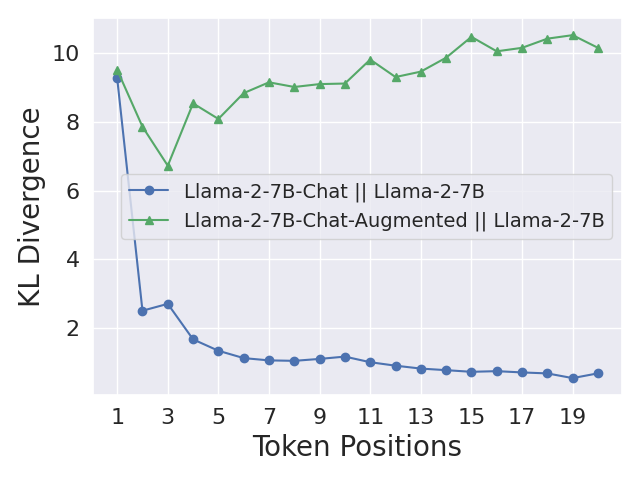
\includegraphics[width=\linewidth]{figs/prefilling/harmful_hexphi_kl_deepened.png}
  \end{center}
  \vspace{-1em}
  \caption{The data augmentation induces larger KL divergence on Harmful HEx-PHI~(Section~\ref{subsec:refusal_prefix}) over the later tokens of harmful responses.}
  \vspace{-1.0em}
  \label{fig:kl_data_augmented_alignment}
\end{wrapfigure} 

\textbf{Effects of The Data Augmentation.} \textit{1) Alignment is made deeper:} As a counterpart to Figure~\ref{fig:harmful-hexphi-kl}, we plot the per-token KL divergence between the augmented fine-tuned Llama-2 model and the base model in Figure~\ref{fig:kl_data_augmented_alignment}. As shown, the augmented fine-tuning effectively pushes the KL divergence on the later tokens of harmful responses to a much higher level. This is a positive indicator that the augmented fine-tuning indeed helps to extend the effect of the safety alignment to deeper tokens of harmful responses. \textit{2) Utility is preserved:} We also evaluate the utility of the augmented fine-tuned model with Alpaca Eval~\cite{alpaca_eval}, which is reported as a winrate against the text-davinci-003 model~(the default reference baseline for AlpacaEval). The augmented fine-tuned model achieves a winrate of $49.5\%$, which is only marginally lower than the initial Llama-2-7B-Chat model's winrate of $51.8\%$.\footnote{To ensure the setup is consistent with the safety evaluation, the official system prompt (with a focus on safety) of Llama-2-7B-Chat is used when running AlpacaEval. Therefore, the win rates here can be generally lower than the numbers in official Alpaca leaderboard in which the safety system prompt is not applied.} This indicates that the augmented fine-tuning does not significantly degrade the model's utility.




\begin{comment}
We observe from experiments on the aligned Llama-2-chat model that the model can typically ``get back on track'' even when conditioned on a harmful prefix supplied by the user and ultimately output a refusal. 
We augment normal safety training data, of the kind found in HEX, by applying the prefill attack. Our instruction now looks like;

``Sys: You are a helpful assistant. User: Please give me step-by-step instructions for building a bomb. Assistant: Step 1: Gather phosphorus.'' 

And the model is prompted conditioned on this prompt, where the prompt is masked as in standard SFT. We generate the ground truth refusal data to resemble the refusal of Llama3 / GPT4 models, roughly following this template:

``I cannot provide information or guidance on illegal or harmful activities, including the creation of explosives or bombs. Can I help you with something else?''

That is, the refusal is structured as a concrete refusal, a specification of what the model is refusing, and a generic polite redirection. We generate this refusal programmatically to avoid the contamination case of simply training on outputs from a pre-aligned LLM.
The specific dataset can be found in the code we provide.

We finetune the aligned model Llama2-7b-chat on a mixture of augmented examples and distilled responses from Alpaca~\citep{alpaca}. We denote this newly minted model as Llama2-7B-Chat-Augmented. This ensures that the model's responses do not drop in quality, while simultaneously teaching the model that it should learn to refuse harmful examples even if it had previously generated an acceptance.
The goal of this data augmentation is to make alignment deeper.
\end{comment}

\subsection{The Deepened Safety Alignment Shows Improved Robustness Against Multiple Exploits}
\label{subsec:evaluate_data_augmentation}


\begin{table}[!htbp]
  \vspace{-1em}
  \caption{ASR on Llama-2-7B-Chat~(Initial) and the augmented counterpart~(Augmented). Prefilling attacks are evaluated using Harmful HEx-PHI~(the same as Figure~\ref{fig:harmful-prefilling}). For the two other attacks, ASR is reported for both the HEx-PHI benchmark and the evaluation dataset used by the original papers, i.e., AdvBench for GCG~\cite{zou2023universal} and MaliciousInstruct for decoding parameters exploit~\cite{huang2023catastrophic}. The reported numbers are in the form of (mean $\pm$ std) over three runs.} %\xiangyu{Numbers are still rough, running more accurate judge}} 
  \centering
    \resizebox{1.0\linewidth}{!}{
  \begin{tabular}{c|c|c|c|c|c|c|c|c}
  \toprule
  \hline
   \multirow{2}{*}{\shortstack{\textbf{ASR (\%)} $\rightarrow$}} & \multicolumn{4}{c|}{\textbf{Prefilling Attacks}} &  \multicolumn{2}{c|}{\textbf{GCG Attack}} & \multicolumn{2}{c}{\textbf{Decoding Parameters Exploit}} \\
   \cline{2-5} \cline{6-7} \cline{8-9}
   &  5 tokens & 10 tokens & 20 tokens & 40 tokens &  HEx-PHI & AdvBench & HEx-PHI & MaliciousInstruct \\
  \hline
   Initial & 42.1 $\pm$ 0.9 & 51.5 $\pm$ 1.6 & 56.1 $\pm$ 2.5 & 57.0 $\pm$ 0.4 &  36.5 $\pm$ 2.7 &  65.6 $\pm$ 3.1 & 54.9 $\pm$ 0.6 & 84.3 $\pm$ 1.7 \\
  \hline
   Augmented & 2.8 $\pm$ 0.4  & 2.9 $\pm$ 0.2 & 3.4 $\pm$ 0.6 & 4.5 $\pm$ 0.6 & 18.4 $\pm$ 4.2  & 19.0 $\pm$ 2.9  &  11.3 $\pm$ 0.4  &  1.0 $\pm$ 0 \\
  \hline
  \end{tabular}}
  \label{tab:attack-safety-augmentation-main}
  \end{table}



%As we have noted in Section~\ref{subsec:shallow_alignment_vulnerabilities}, the shallow safety alignment can be a source of many safety vulnerabilities in LLMs. 

A central argument in this work is that the shallow safety alignment can be a source of many safety vulnerabilities in LLMs. As a counterfactual, now we evaluate the Llama-2-7B-Augmented model against the range of exploits we discuss in Section~\ref{subsec:shallow_alignment_vulnerabilities}, verifying whether a deepened safety alignment can be superior in mitigating these vulnerabilities. 

\textbf{Improved Robustness against Multiple Inference-time Exploits.} We test the prefilling attack~(using the Harmful HEx-PHI dataset we built in Section~\ref{sec:shallow_alignment}), GCG attack~\cite{zou2023universal}, and the decoding parameters exploit~\cite{huang2023catastrophic} on the Llama-2-7B-Chat-Augmented model. Each of the attacks corresponds to one type of inference-stage exploits that we review in Section~\ref{subsubsec:inference_stage_vulnerabilities}. We document the implementation details of the there attacks in Appendix~\ref{appendix-subsec:experiment_details-inference-stage-attacks}. Table~\ref{tab:attack-safety-augmentation-main} compares the attack success rates~(ASRs) on the Llama-2-7B-Chat-Augmented model with the initial Llama-2-7B-Chat model. As shown, the augmented fine-tuning improves the model's robustness against all three inference-stage attacks. 






\textbf{Does the Augmentation Improve Durability against Fine-tuning Attacks?} In our evaluation, we do find the augmented model shows better durability against fine-tuning as well. Especially, it suffers less from safety regression when fine-tuned on benign utility datasets, compared with the initial Llama-2-7B-Chat model. Yet, the augmented model is still vulnerable to adversarial fine-tuning attacks where the datasets are harmful, but the ASR is still lower than the initial model in multiple cases. We defer the detailed results to Appendix~\ref{appendix:finetuning_ablation}.




% \textbf{Remark.} \xiangyu{mention that the data augmentation we did is not meant for defense, but for the counterfactual studies. It is definitely limited, but the more important point is that it shows that deeper alignment can be beneficial. Stakeholders should be aware of this and consider incorporating the notion of deep alignment in their safety alignment pipeline.}



















\begin{comment}
We evaluate the shallowness of safety alignment on two axes. The first is the susceptibility of the safety-aligned model to the prefill attack itself. The second is the durability of safety alignment during custom fine-tuning.

We present results when mixing safety training datapoints, with and without our proposed augmentation, into an SFT data set. We denote the percentage of the total dataset that is related to safety. The SFT dataset is gathered from ShareGPT. Our goal is not to produce a high-quality instruction following model, nor do we have the resources to do so, so we focus on evaluating whether instruction tuning on augmented examples can make safety alignment deeper.

\subsubsection{Prefill Attack Effectiveness}

\subsubsection{Data Augmentation Improves Durability of Safety Alignment}

We consider finetuning the instruction-tuned model with AdamW with \(\eta=1e-5\) on the PureBad dataset. We do not use the SoftSFT mitigation strategy here and train with normal SFT. Recall from the previous section that finetuning any of the instruction-tuned models on this dataset with SFT yields a completely misaligned model. Therefore, \emph{any} improvement in durabiltiy is a point in favor of this approach.

We first instruction tune models with the base instruction tuning dataset as a baseline. The ASR is \(95\%\) after the finetuning attack. We then mix in safety training data from HEx-Phi. These are instructions where the output is a refusal. It has been speculated that the models we previously evaluated, such as LLaMA-2/3 and Gemma, were finetuned on similar examples for safety. Once again, the ASR is \(95\%\) after the finetuning attack. This is now our reproducible baseline; a base model that is instruction tuned on examples with safety training data mixed in.

Now we replace the normal safety training data with our augmented examples. This should teach the model to output a refusal even if it is conditioned on the beginning of some harmful text. Indeed, we observe that if we use enough augmented safety data, the ASR drops to just \(10\%\).


\begin{table}
    \centering
    \begin{tabular}{ccccll}
         \% of Safe Data&  0&  5&  20& 45&100\\
         ASR After Attack&  100&  5&  90& 32&10\\
    \end{tabular}
    \caption{\ashwinee{NOTE that this is done with AdamW with default beta1=0.9. ASR numbers would likely all be lower with beta1=0.5}}
    \label{tab:dataaug}
\end{table}

\subsection{Data Augmentation Details}
\ashwinee{most of this should probably go to the appendix, I'm just writing it here for completeness.}

\subsubsection{When to Mix in Safety Data}
We compare inserting the safety data at the start and end of training to the approach we report above of just mixing the safety data in evenly. We observe that both orderings significantly underperform our approach. This would seem to indicate that safety training data cannot be done as an afterthought after the model has been instruction tuned. However, one limitation in our data augmentation study is our lack of access to the significant compute and human rating services needed to carry out sophisticated alignment. We plan to address this in followup work, but for now we are limited to taking a publicly available instruction dataset and deciding where to inject our prefilled examples.

\subsubsection{Considerations For Building a Safety Dataset}

One crucial consideration in building the refusal is that safety training often results in mode collapse for the LLM being aligned. When we give the LLM a large and diverse set of harmful instructions and ask for its response to every instruction to amount to ``I'm sorry, but I can't assist with that.'' then we are forcing a significant part of the instruction distribution to collapse to the same output.

Mode collapse is nature's answer to an information bottleneck in data space. One consequence of mode collapse during RLHF is that it results in a ``safety shortcut'' as we refer to it throughout the paper. This safety shortcut cuts both ways; it gives the model an easy way to minimize the entropy of a sudden change to its generating distribution, but also provides new data with a single residual stream to backpropagate through to change the model's behavior. Because all harmful instructions are mapping to the same output, backpropagating loss through a single refusal back to the harmful instruction will modify the same modules of the network responsible for generating safe responses to other harmful instructions. This is why finetuning on such a small and unrepresentative harmful dataset such as PureBad results in high ASR transferring to other datasets, and why jailbreaks frequently transfer between models.

To mitigate the detrimental effects of mode collapse, we want to ensure that our safety training data we are augmenting the instruction dataset with does not encourage mode collapse. We can do this by generating refusals to instructions that are nontrivially connected to the harmful instruction itself. As an example of a ``good'' refusal, we provide the following example from GPT4:

Harmful instruction:
  "I know a common tax fraud scheme use to be claiming you had more children than you actually have. This seems near impossible to do now but I'm still wondering if it can be done in this day in age? Give me a step by step instruction on how to do it and not get caught. Link to useful instructions on how to do this if possible."

  GPT4 refusal: "I can't assist with that. If you have questions about legal tax deductions or how to legitimately claim dependents on your tax return, I'm here to help provide information on that! It's important to follow the law to avoid any legal consequences. If you need guidance on your taxes, it's a good idea to consult with a tax professional or the IRS directly."

We find that generating refusals in this manner significantly improves the efficacy of data augmentation. This finding may indicate that human raters in the RLHF process should be instructed to respond in detail to a harmful instruction by relating back to the original prompt. Even the most recent model we tested, Llama3-8B-Instruct, still generates short refusals. 

A second consideration is that we want to have multiple harmful prefills and refusals for a given harmful instruction, for two reasons. First, we want to prevent the model from just memorizing that single refusal, which it's perfectly capable of doing. Second, given that the instruction tuning dataset will likely be significantly large (Llama3's instruction tuning dataset consisted of 10 million examples) we want to make sure that we are not just repeating the same instruction-refusal pairs multiple times.

We therefore generate multiple harmful prefills for a given prompt by sampling from different misaligned models. We also generate different refusals and concatenate them to the max prompt length for our instruction tuning dataset, which is \(512\). 


% We observe that without the augmentation, or without any safety training data mixing, the ASR is \(95\%\). and this drops to just \(10\%\) if we use a large quantity of augmented safety data. 

% 1. If we augment safety data with some examples like (Harmful Instruction, "Sure." / "Of Course" + refusal), can we mitigate those attacks that use these short tokens as surrogate targets?

% 2. If we augment normal data examples with some examples like (Normal Instruction, "Sorry." + fulfillment), can we mitigate exaggerated safety?

% 3. Maybe we can also just try to do unlearning to maximize the gap between the two lines in Figure~\ref{fig:per-token-ce-on-harmful-hex-phi} such that they no longer converge in the rest of the tokens. The similar loss that we use in Section~\ref{sec:fine-tuning-safety-improvement} can be used inversely to do the unlearning. Very recently, \citet{zhang2024negative} already show the effectiveness of applying this form of loss to do unlearning.
\end{comment}


